%\documentclass[mathserif]{beamer}
\documentclass[handout]{beamer}
%\usetheme{Goettingen}
\usetheme{Warsaw}
%\usetheme{Singapore}
%\usetheme{Frankfurt}
%\usetheme{Copenhagen}
%\usetheme{Szeged}
%\usetheme{Montpellier}
%\usetheme{CambridgeUS}
%\usecolortheme{}
%\setbeamercovered{transparent}
\usepackage[english, activeacute]{babel}
\usepackage[utf8]{inputenc}
\usepackage{amsmath, amssymb}
\usepackage{dsfont}
\usepackage{graphics}
\usepackage{cases}
\usepackage{graphicx}
\usepackage{pgf}
\usepackage{epsfig}
\usepackage{amssymb}
\usepackage{multirow}	
\usepackage{amstext}
\usepackage[ruled,vlined,lined]{algorithm2e}
\usepackage{amsmath}
\usepackage{epic}
\usepackage{epsfig}
\usepackage{fontenc}
\usepackage{framed,color}
\usepackage{palatino, url, multicol}
\usepackage{listings}
%\algsetup{indent=2em}
\newcommand{\factorial}{\ensuremath{\mbox{\sc Factorial}}}
\newcommand{\BIGOP}[1]{\mathop{\mathchoice%
{\raise-0.22em\hbox{\huge $#1$}}%
{\raise-0.05em\hbox{\Large $#1$}}{\hbox{\large $#1$}}{#1}}}
\newcommand{\bigtimes}{\BIGOP{\times}}
\vspace{-0.5cm}
\title{Deisgn of Experiments \& Hypothesis Testing}
\vspace{-0.5cm}
\author[Felipe Bravo Márquez]{\footnotesize
%\author{\footnotesize  
 \textcolor[rgb]{0.00,0.00,1.00}{Felipe José Bravo Márquez}} 
\date{ \today }






\begin{document}
\begin{frame}
\titlepage


\end{frame}


%%%%%%%%%%%%%%%%%%%%%%%%%%%

% Useful references: http://www.buders.com/UNIVERSITE/Universite_Dersleri/istatistik/sampling_distributions_and_point_estimation_of_parameters.pdf
% http://homepage.divms.uiowa.edu/~rdecook/stat2020/notes/ch7_pt1.pdf


\begin{frame}{Motivation}
\scriptsize{


In the first lecture we discussed the three major goals of statistics:
\begin{enumerate}
 \item Describe
 \item Decide
 \item Predict 
\end{enumerate}



 \begin{itemize}
  \item In this lecture we will introduce the ideas behind the use of statistics to make decisions.
  \item In particular, decisions about whether a particular \textbf{hypothesis} is supported by the data. \cite{poldrack2019statistical}
 \end{itemize}

} 
\end{frame}



\begin{frame}{Null Hypothesis Statistical Testing (NHST)}
\scriptsize{
\begin{itemize}
 \item The specific type of hypothesis testing that we will discuss is known null hypothesis statistical testing (NHST).
\item  If you pick up almost any scientific research publication, you will see NHST being used to test hypotheses.
\item Learning how to use and interpret the results from hypothesis testing is essential to understand the results from many fields of research.
\item NHST is usually applied to \textbf{experimental} data.
\item Thus, we need to introduce basic concepts on the design of experiments.
\end{itemize}



} 
\end{frame}

\section{Experiments}

\begin{frame}{Experiments and Inference About Cause}
\scriptsize{
\begin{itemize}
 \item In the previous lecture we studied how to infer characteristics of a population from sample data using surveys or polls.
 \item A second type of inference is when we want to infer \textbf{cause-effect relationships} between two or more variables (e.g, does smoking cause cancer) from experimental data. 
 \item Example \cite{watkins2010statistics}: Children who drink more milk have bigger feet than children who drink less milk. 
 
 
\end{itemize}


\begin{figure}[h!]
	\centering
	
\includegraphics[scale=0.25]{pics/milk.png}
	\caption{Image source: \url{https://www.dreamstime.com}}
\end{figure}



} 
\end{frame}


\begin{frame}{Experiments and Inference About Cause}
\scriptsize{

\begin{itemize}
\item There are three possible explanations for this association:
 \begin{enumerate}
 \scriptsize{
 \item Drinking more milk causes children’s feet to be bigger.\\
	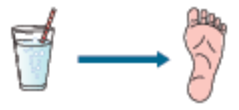
\includegraphics[scale=0.25]{pics/cause1.png}

 
 \item Having bigger feet causes children to drink more milk. \\
 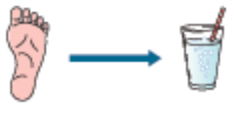
\includegraphics[scale=0.25]{pics/cause2.png}
 
 \item A \textbf{lurking variable} is responsible for both. \\
 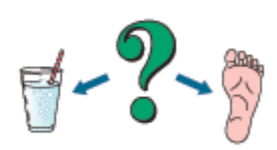
\includegraphics[scale=0.25]{pics/cause3.png}
 }
\end{enumerate}


 \item A lurking variable is a variable that may or may not be apparent at the outset but, once identified, could explain the pattern between the variables.

\item We know that bigger children have bigger feet, and they drink more milk because they eat and drink more of everything than do smaller children.


\end{itemize}



} 
\end{frame}



\begin{frame}{Experiments and Inference About Cause}
\scriptsize{

\begin{itemize}

\item The right explanation is the third one: the child's \textbf{overall size} is the lurking variable.

 \item However, suppose we want to prove that explanation 1 is the right reason with the following approaches. 
 \item Approach 1: take a bunch of children, give them milk, and wait to see if their feet grow.
 \item This won't prove anything, because children's feet will grow whether they drink milk or not.
 \item Approach 2: take a group of children, divide them randomly into two \textbf{groups}: 1) one group that will drink milk and 2) another group that will not, wait and compare the size of the feet of both groups. 
 \item This approach is an \textbf{experiment}, and is the only way to establish cause and effect.
 
\end{itemize}



} 
\end{frame}


\begin{frame}{Main Concepts of Experimental Design}
\scriptsize{


\begin{itemize}
 \item \textbf{Experimental units}: the subjects on which we experiment (e.g, patients, users, laboratory animals). When the experiment units are people, we call them  \textbf{subjects}.
 \item \textbf{Treatments}: the conditions on which we compare different unit groups. Examples: drinking milk vs. not drinking milk, smoking vs. not smoking, taking drug A vs. drug B.
 \item \textbf{Treatment or Experimental group}: a group of units receiving a particular treatment. Example: patients taking a new drug, software users seeing a new layout.
 \item \textbf{Control group}: a group of units used for comparison receiving either a standard treatment or no treatment at all. Example: patients taking a placebo (a fake treatment), software users seeing the standard layout.
 
  \item \textbf{Response variable}: the variable of interest used to measure the effect of the treatments on the units. Examples: weight, birth rate, antibody levels, click-rate, revenue, etc.
 
\end{itemize}



} 
\end{frame}


\begin{frame}{Main Concepts of Experimental Design}
\scriptsize{


\begin{itemize}

 \item \textbf{Randomization}: random assignment of treatments (including the control group) to units. This is very important since not all units are alike (e.g., people have different ages, weights, preferences). \\
 \begin{itemize}
 \scriptsize{
  \item  Randomization is the most reliable method of creating homogeneous treatment groups, without involving any potential biases or judgments.
 }
 \end{itemize}


  \item \textbf{Replication}: the repetition of an experiment on a large group of subjects. Replication reduces variability in experimental results. 
  
  \item \textbf{Randomized Controlled Trial} (RCT): an experiment in which units are randomly assigned to one of several treatments and one of these groups is a control group.
  
  \item \textbf{Blind Experiment}:  when the units (e.g., patients) don't know the treatment they are receiving.
  
  \item \textbf{Double-blind Experiment}: when neither the units (e.g., patients) nor the experimenters (e.g., doctors) know who is receiving a particular treatment.
  
\end{itemize}



} 
\end{frame}


\begin{frame}{Main Concepts of Experimental Design}
\scriptsize{

\begin{figure}[h!]
	\centering
	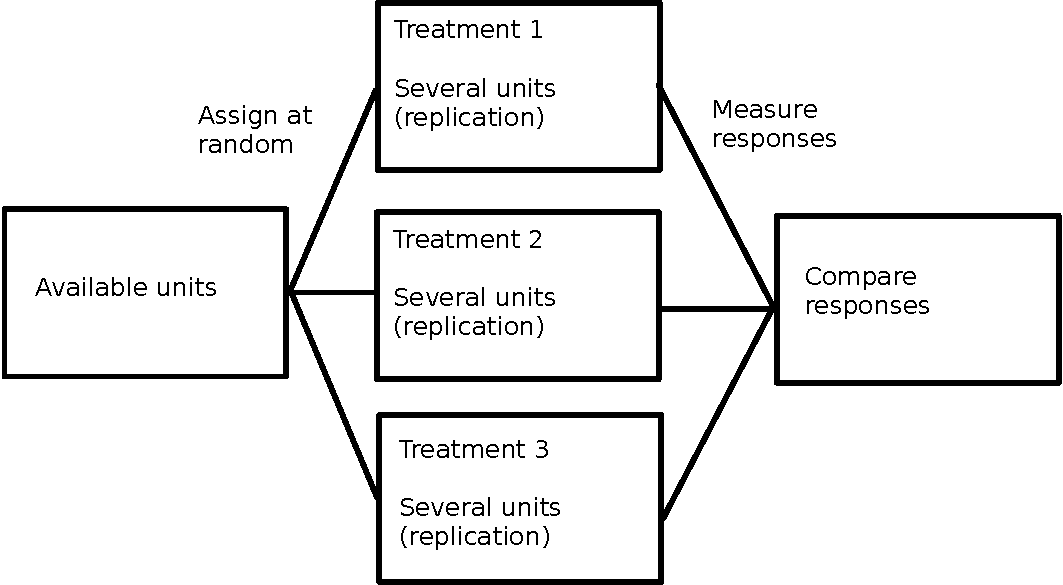
\includegraphics[scale=0.6]{pics/experiment.pdf}
\end{figure}

Characteristics of a well-desgined experiment.


} 
\end{frame}


\begin{frame}{A/B Testing}
\scriptsize{


\begin{itemize}

\item Data-driven companies like Amazon, Microsoft, eBay, Facebook, Google and Netflix often conduct experiments to make decisions \cite{kohavi2012trustworthy}.

\item In this context, experiments are called \textbf{online  controlled experiments} or \textbf{A/B tests}. 
 

 \item The idea is the same, users (experimental units) are randomly exposed to one of two variants of a webpage or APP: Control (A), or Treatment (B).
 
 \item When the number of variants (treatments) is greater we have an A/B/n test.
 
 \item The response variable is called \textbf{Overall  Evaluation  Criterion} (OEC), which is  a  quantitative measure of the experiment's objective. 
 
 \item OECs can be revenue, clickthrough-rate, user session duration, etc...
 \end{itemize}

} 
\end{frame}


\begin{frame}{A/B Testing}

 \begin{figure}[h!]
	\centering
	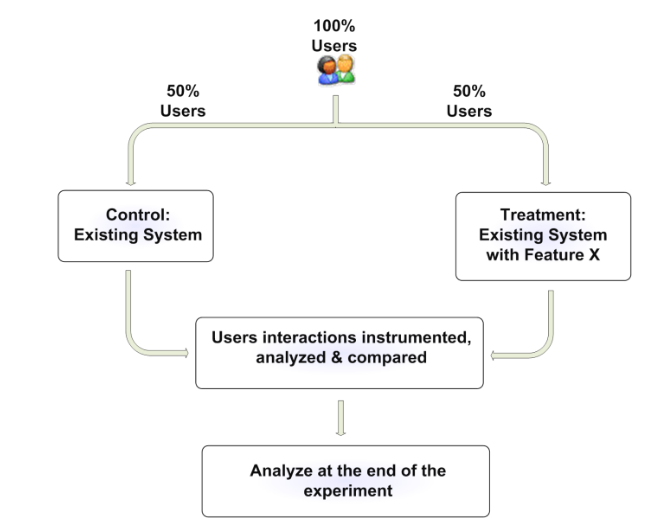
\includegraphics[scale=0.34]{pics/abtest.png}
\end{figure}
Image souce: \cite{kohavi2012trustworthy} 
\end{frame}



\begin{frame}{Example: MSN Real Estate}
\scriptsize{


\begin{itemize}

\item The team running the MSN Real Estate site wanted to test different designs for the ``Find a home'' widget \cite{kohavi2009online}.

\item Visitors who click on this widget are sent to partner sites, and Microsoft receives a referral fee. 

\item Six different designs of this widget, including the incumbent (control), were proposed.

\item Users were randomly splited between the variants in a persistent manner (a user receives the same experience in multiple visits) during the experiment period.

\end{itemize}



} 
\end{frame}


\begin{frame}{Example: MSN Real Estate}


\begin{figure}[h!]
	\centering
	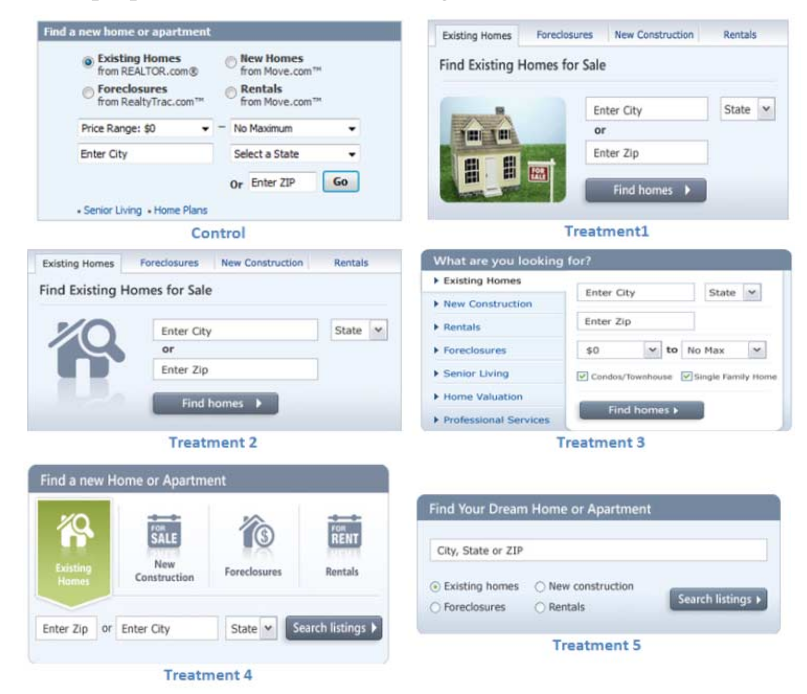
\includegraphics[scale=0.4]{pics/widgets.png}
\end{figure}




\end{frame}


\begin{frame}{Example: MSN Real Estate}
\scriptsize{


\begin{itemize}


 
 \item Their interactions are instrumented and key metrics computed. 
 
 \item In this experiment, the Overall Evaluation Criterion (OEC) was simple: average revenue per user.
 \item The winner, Treatment 5, increased revenues by almost 10\% (due to increased clickthrough).
 
 \item The Return-On-Investment (ROI) for MSN Real Estate was phenomenal, as this is their main source of revenue, which increased significantly through a simple change.

\end{itemize}



} 
\end{frame}




\begin{frame}{Observational Studies and Confounding}
\scriptsize{

\begin{itemize}

 \item Sometimes we can't randomly assign units to the different treatments.
 
 \item For example, it would be unethical to design a randomized controlled trial deliberately exposing people to a potentially harmful situation. 
 
 \item In an \textbf{obervational study} the conditions of interest are aready built into the units being studied.
 
 \item Observational studies are almost always worse than controlled experiments for determining cause-effect relationships.
 
 \item But sometimes is the only thing we can do.
 
 \item A phenomenum called \textbf{confounding} is the major treat to observational studies.
 
 \item Two possible influences on an observed outcome are \textbf{confounded} if they are mixed together in a way that makes it impossible to separate their effects on the responses \cite{watkins2010statistics}.
  
\end{itemize}



} 
\end{frame}

\begin{frame}{Example of Confounded Observational Study}
\scriptsize{

\begin{itemize}

 \item The thymus, a gland in your neck, behaves in a peculiar way. 
 
 \item Unlike other organs of the body, it doesn't get larger as you grow—it actually gets smaller. 
 \item Ignorance of this fact led early 20th-century surgeons to adopt a worthless and dangerous surgical procedure.
 
 \begin{figure}[h!]
	\centering
	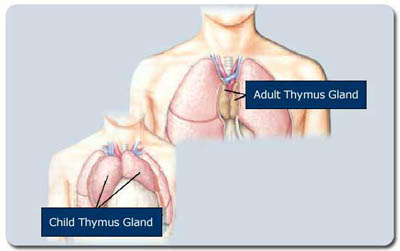
\includegraphics[scale=0.4]{pics/ThymusSizeDiagram.jpg}
	\caption{source: \url{http://esvc001414.wic005tu.server-web.com/tech_imm_bio_principle.htm}}
\end{figure}
 
  
\end{itemize}



} 
\end{frame}


\begin{frame}{Example of Confounded Observational Study}
\scriptsize{

\begin{itemize}

 \item Many infants were dying of what seemed to be respiratory obstructions.
 
 \item Doctors did autopsies on infants who died with respiratory symptoms and compared againts aotopsies made on adults who died of various causes.

\item Most autopsies to infants show big thymus glands compared to adults.

\item Doctors concluded that the respiratory problems were caused by an enlarged thymus. 


\item In 1912, Dr. Charles Mayo published an article recommending removal of the thymus to treat respiratory problems in children. 

\item This recommendation was made even though a third of the
children who were operated on died. 
  
\item The doctors could not tell whether children with a large thymus tended to have more respiratory problems because they had no evidence about children with a smaller thymus.  
  
\end{itemize}



} 
\end{frame}



\begin{frame}{Example of Confounded Observational Study}
\scriptsize{

\begin{itemize}


\item Age and size of thymus were confounded.

\item The thymus study is an example of an observational study, not an experiment.

\begin{table}
\center
 \begin{tabular}{|c|ccc|}  \hline
 
& & \multicolumn{2}{c|}{Age} \\ \hline
& & Child & Adult \\
\multirow{2}{*}{ Thymus size } & Large & Problems & No evidence \\ 
& Small & No evidence & No problems \\ \hline
\end{tabular} 
\end{table}

\item If Dr. Mayo had used a randomized experiment to evaluate surgical removal of the thymus, he would have seen that the treatment was not effective and many lives might have been
spared. 
\item However, at the time, randomized experiments were not often used in the medical profession.
  
\item These days, any new medical treatment (e.g., a COVID vaccine) must prove its value in an RCT.  
\end{itemize}



} 
\end{frame}

\begin{frame}{Another Example of Confounding}
\scriptsize{

\begin{itemize}

\item Suppose we want to compare student performance on standardized tests (e.g., SIMCE, PSU) in public and private schools.

\item We know that the socioeconomic distribution of students is different in public and private schools.

\item We also suspect that socioeconomic background may influence student performance on these tests.

\item The type of school (public or private) and the socioeconomic background are confounded.
  
\end{itemize}



} 
\end{frame}



\begin{frame}{Randomized Paired Comparison (Matched Pairs)}
\scriptsize{

\begin{itemize}

\item Randomized Paired Comparison or Matched Pairs is an approach to design experiments \textbf{controlling} for confounding variables. 

\item We sort the experimental units into pairs of similar units (matched pairs), where similarity is measured according to confounding variables.

\item  The two units in each pair should be enough alike that you expect them to have a similar response to any treatment.

\item Randomly decide which unit in each pair is assigned which treatment.

\item We are essentially building comparable Control and Treatment populations by segmenting the users by common confounds, similarly to stratified sampling.
  
\end{itemize}



} 
\end{frame}


\begin{frame}{Matched Pairs Example}
\scriptsize{

\begin{itemize}

\item Suppose we want to study the relation between hypertension and end-stage renal disease (ESRD) \cite{de2011matching}.

\item Obesity is a potential confounder as obesity is associated with both hypertension and ESRD. 

\item Matching approach: we ensure that the average body mass index (BMI) is the same in the group of patients exposed to hypertension and another group of patients unexposed to hypertension. 

\item This could be achieved by searching an obese patient without hypertension for each obese patient with hypertension.
  
\item Other potential confouding variables like age or sex could also be considered in the matching.  
  
\end{itemize}



} 
\end{frame}


\section{Hypothesis Testing}

\begin{frame}{Hypothesis Testing}
\scriptsize{
\begin{itemize}
 \item When we want to test whether some assumed \textbf{property} about a population is contrasted with a statistical sample we use a \textbf{hypothesis test}.
\item The test consists of the following hypotheses:
 \begin{itemize}
\scriptsize{
\item \textbf{Null Hypothesis} $H_{0}$: Symbolizes the current situation. What has been considered real up to the present.
\item \textbf{Alternative Hypothesis} $H_{a}$: it is the alternative model that we want to consider. 
}
 \end{itemize}
\item The idea is to find enough \textbf{statistical evidence} to reject $H_{0}$ and be able to conclude $H_{a}$.
\item If we do not get enough statistical evidence \textbf{we fail to reject} $H_{0}$

\end{itemize}



} 
\end{frame}



\begin{frame}{Hypothesis Testing}
\scriptsize{

\begin{block}{Methodology to Perform a Hypothesis Test}
\begin{itemize}
 \item Choose a null hypothesis $H_0$ and alternative $H_a$.
 \item Set a test significance level $\alpha$.
 \item Calculate a statistic $T$ from the data.
 \item  The statistic $T$ is usually a standardized value that we can check in a distribution table.
 \item Define a rejection criterion for the null hypothesis. It is usually a critical value $c$.
\end{itemize}
\end{block}



} 
\end{frame}


\begin{frame}{Types of T-tests}
 \scriptsize{
\url{https://en.wikipedia.org/wiki/Student\%27s_t-test}
\begin{itemize}
 \item Single-sample t-test
 \item Unpaired two sample t-test: better using \url{https://en.wikipedia.org/wiki/Welch\%27s_t-test}
 \item Paired two sample t-test
\end{itemize}

\url{https://www.datanovia.com/en/lessons/types-of-t-test/\#one-sample-t-test}
}
Tests can be one-sided or two-sided

Nice explanations of degrees of freedom: \url{https://crumplab.github.io/statistics/t-tests.html}

\end{frame}



\begin{frame}[fragile]{Single-sample T-test}
\scriptsize{
\begin{itemize}
 \item Example: It is known that the average number of hours of monthly Internet use in Chile is 30 hours.
 \item Suppose we want to show that the average is different from that value.
 \item We would have that $H_0: \mu=30$ and $H_{a}: \mu \neq 30$
 \item Let's set $\alpha=0.05$ and collect 100 observations.
 \item Suppose we get $\overline{X_{n}}=28$ and $s=10$
 \item  One way to test is to construct a confidence interval for $\mu$ and see if $H_{0}$ is in the interval.
\begin{verbatim}
> 28-qt(p=0.975,99)*10/sqrt(100)
[1] 26.01578
> 28+qt(p=0.975,99)*10/sqrt(100)
[1] 29.98422 
\end{verbatim}
\item The interval would be the acceptance zone of $H_0$ and anything outside of this would be my rejection region.
\item Since 30 is in the rejection region, I reject my null hypothesis with $5\%$ confidence.
\end{itemize}



} 
\end{frame}


\begin{frame}[fragile]{Univariate T-test}
\scriptsize{
\begin{itemize}
 \item Another way to perform the test is to compute the statistic  $T=\frac{\overline{X_{n}}-\mu_{o}}{\frac{s}{\sqrt{n}}}$
 \item  In this case it would be \begin{displaymath}
                           T=\frac{28-30}{\frac{10}{\sqrt{100}}}=-2
                          \end{displaymath}
\item Since $H_{a}: \mu \neq 30$, we have a two-sided test, where the acceptance region is.
\begin{displaymath}
 t_{n-1,1-\alpha/2}<T<t_{n-1,\alpha/2}
\end{displaymath}
\begin{verbatim}
 > qt(0.025,99)
[1] -1.984217
> qt(0.975,99)
[1] 1.984217
\end{verbatim}
\item Since $T$ is in the rejection region, we reject the null hypothesis.

\end{itemize}



} 
\end{frame}


\begin{frame}[fragile]{P-value}
\scriptsize{
\begin{itemize}
 \item Generally, in addition to knowing whether we reject or fail to reject a null hypothesis we want to quantify the evidence we have against it.
 \item A \textbf{p-value} is defined as the probability of obtaining an outcome at least as extreme as that observed in the data given that the null hypothesis is true.
 \item ``Extreme'' means far from the null hypothesis and favorable for the alternative hypothesis.
 \item If the \textbf{p-value} s less than the significance level $\alpha$, we reject $H_{0}$ 
 \item Example:
\begin{verbatim}
> data(iris)
> mu<-3 # null hypothesis
> alpha<-0.05
> n<-length(iris$Petal.Length)
> xbar<-mean(iris$Petal.Length)
> s<-sd(iris$Petal.Length)
> se<-s/sqrt(n)
> t<-(xbar-mu)/(s/sqrt(n))
> pvalue<-2*pt(-abs(t),df=n-1)
> pvalue
[1] 4.94568e-07 # is less than 0.05 then we reject H0
\end{verbatim}
\end{itemize}

 


}
\end{frame}

\begin{frame}[fragile]{Univariate T-test}
\scriptsize{
\begin{itemize}
 \item The elegant way to do it in R:
\end{itemize}

\begin{verbatim}
> t.test(x=iris$Petal.Length,mu=3)

	One Sample t-test

data:  iris$Petal.Length 
t = 5.2589, df = 149, p-value = 4.946e-07
alternative hypothesis: true mean is not equal to 3 
95 percent confidence interval:
 3.473185 4.042815 
sample estimates:
mean of x 
    3.758 
\end{verbatim}
}



\end{frame}

\begin{frame}{Errors}
 \scriptsize{

\begin{itemize}
 \item We have two types of errors when we perform a hypothesis test
 \item Type I error: it is when we reject the null hypothesis when it is true.
 \item This error is equivalent to the significance level $\alpha$. 
 \item Type II error: is when the null hypothesis is false but we do not have statistical evidence to reject it.
 \item To mitigate type I errors we generally use smaller values of $\alpha$.
 \item To mitigate type II errors we generally work with larger samples.
 \item There is a trade-off between type I and type II errors. 
\end{itemize}

 \begin{table}
\begin{tabular}{c | c c}
\hline
  & Retain $H_0$ &  Reject $H_{0}$   \\ 
\hline
$H_0$ true & \checkmark & type I \\
$H_1$ true & type II error & \checkmark \\
\hline
\end{tabular}
\end{table}

}
\end{frame}




\begin{frame}{Statistical Power}
 
\end{frame}

\begin{frame}{Critics to Hypothesis Testing}
 
\end{frame}


\begin{frame}{FOUR CARDINAL RULES OF STATISTICS by Daniela Witten}
\scriptsize{
\begin{itemize}
% source: https://twitter.com/daniela_witten/status/1312180955801505794
 \item ONE:  CORRELATION DOES NOT IMPLY CAUSATION.  Yes, I know you know this, but it’s so easy to forget! Yeah, YOU OVER THERE, you with the p-value of 0.0000001 — yes, YOU!! That’s not causation.
 \item No matter how small the p-value for a regression of IQ onto shoe size is, that doesn’t mean that big feet cause smarts!!  It just means that grown-ups tend to have bigger feet and higher IQs than kids.
 \item So, unless you can design your study to uncover causation (very hard to do in most practical settings — the field of causal inference is devoted to understanding the settings in which it is possible), the best you can do is to discover correlations.  Sad but true.
 \item TWO:  A P-VALUE IS JUST A TEST OF SAMPLE SIZE.  Read that again — I mean what I said!  If your null hypothesis doesn't hold (and null hypotheses never hold IRL) then the larger your sample size, the smaller your p-value will tend to be.
 \item If you’re testing whether mean=0 and actually the truth is that mean=0.000000001, and if you have a large enough sample size, then YOU WILL GET A TINY P-VALUE.
 \item Why does this matter? In many contemporary settings (think: the internet), sample sizes are so huge that we can get TINY p-values even when the deviation from the null hypothesis is negligible. In other words, we can have STATISTICAL significance w/o PRACTICAL significance.
 \end{itemize}

} 
\end{frame}

\begin{frame}{FOUR CARDINAL RULES OF STATISTICS by Daniela Witten}
\scriptsize{
\begin{itemize}
 \item Often, people focus on that tiny p-value, and the fact that the effect is of **literally no practical relevance** is totally lost.
 \item This also means that with a large enough sample size we can reject basically ANY null hypothesis (since the null hypothesis never exactly holds IRL, but it might be “close enough” that the violation of the null hypothesis is not important). 
 \item Want to write a paper saying Lucky Charms consumption is correlated w/blood type? W/a large enough sample size, you can get a small p-value.  (Provided there’s some super convoluted mechanism with some teeny effect size… which there probably is, b/c IRL null never holds)
\item THREE:  SEEK AND YOU SHALL FIND. If you look at your data for long enough, you will find something interesting, even if only by chance! 
In principle, we know that we need to perform a correction for multiple testing if we conduct a bunch of tests.
\item But in practice, what if we decide what test(s) to conduct AFTER we look at data?  Our p-value will be misleadingly small because we peeked at the data.  Pre-specifying our analysis plan in advance keeps us honest… but in reality, it’s hard to do!!!
\item Everyone is asking me about the mysterious and much-anticipated fourth rule of statistics. The answer is simple: we haven’t figured it out yet.... that’s the reason we need to do research in statistics
\end{itemize}

} 
\end{frame}


%%%%%%%%%%%%%%%%%%%%%%%%%%%
%%%%%%%%%%%%%%%%%%%%%%%%%%%
\begin{frame}[allowframebreaks]\scriptsize
\frametitle{References}
\bibliography{bio}
\bibliographystyle{apalike}
%\bibliographystyle{flexbib}
\end{frame}  









%%%%%%%%%%%%%%%%%%%%%%%%%%%

\end{document}
